\documentclass{beamer} %for at du kan lave en pr�sintation skal du skriove beamer i class% 
\usetheme{Marburg} %her bestemmer du designet fx madrig du kan ogs� bestemme om der skal vises under katagorier%
\setcounter{tocdepth}{1}

\usepackage[latin1]{inputenc} %standart%
\usepackage[english]{babel}%standrat%
\usepackage{amsmath,amsfonts,amssymb}%standrat%
\usepackage[]{subfig}

\usepackage{tabularx}
\usepackage[]{graphicx}
\usepackage{movie15}
\usepackage{tikz} 

\usepackage{listings}


\usepackage{color}

\newcommand{\titlename}{Implementering af Aalborg Modellen for Problembaseret L�ring i Moodle}

\definecolor{light-gray}{gray}{0.80}
\definecolor{gray95}{gray}{.95}
\definecolor{gray92}{gray}{.92}
\definecolor{gray75}{gray}{.75}
\definecolor{gray45}{gray}{.45}

\lstdefinestyle{sourceCode}
{ 
	numbers=left,
	numbersep=5pt, 
	stepnumber=1,
	captionpos=b,  %bottom
	keywordstyle=\color[rgb]{0,0,1},
	commentstyle=\color[rgb]{0.133,0.545,0.133},
	stringstyle=\color[rgb]{0.627,0.126,0.941},
	%backgroundcolor=\color{gray95},
	%frame=lrtb,
	framerule=0.5pt,
	linewidth=1.00\textwidth,
	tabsize=4,
	numberbychapter=true,
	basicstyle=\ttfamily\footnotesize,
	language=C,
	breaklines=true,
	showstringspaces=false,
	emph=[1]{endregion,region,get,set,enum},%%%%%%%%%%% Add new keywords here
	%emph=[2]{Tag,Problem,Person,List,NotSupportedException,TestMethod,ProblemSearch,Assert,
	%EntityCollection,Department,IEnumerable,TimeSpan,DateTime},%%Classes
	emphstyle=[1]{\color[rgb]{0,0,1}},
	emphstyle=[1]{\color[rgb]{0,0,1}},
	emphstyle=[2]{\color[rgb]{0.1,0.5,0.5}},
	float=htb,
	breakindent=20pt
}






\author{SW608F12}
\institute{Aalborg University}
\title{\titlename}
\subtitle{Applikantionsudvikling}


\begin{document}
	\begin{center}
	\parbox{\textwidth}{
		\begin{center}

			\thispagestyle{empty}

			\LARGE
			AALBORG UNIVERSITY \\


			STUDENT REPORT \\
			sw608f12 \\ 
			
			\vspace{10mm}
			
			\begin{figure}[H]%
			\centering
			\LARGE
			\begin{tabular}{ c }
			\hline \\
				\textbf{Implementing the} \\
				\textbf{Aalborg Problem Based Learning Model} \\ 
				\textbf{in Moodle} \\ \\
			\hline 
			\end{tabular}
			\end{figure}

			Theme: \\
			Application Development \\
			 
			\vspace{10mm}
			Authors: \\
			Alex Bondo Andersen\\
			Kim Ahlstr\o{}m Jakobsen\\
			Mikael Midtgaard\\
			Rasmus Veiergang Prentow\\ 
			
			
		
			

		\end{center}		
	}
\end{center}
	
	\newcommand{\reqs}{Systemkrav}
\newcommand{\slutbrugere}{Slutbrugere}
\newcommand{\funcreqs}{Funktionelle}
\newcommand{\nonfuncreqs}{Ikke-Funktionelle}
%\newcommand{\nonfuncreqs}{Kvalitetskrav}

\newcommand{\admreq}{Administration af Projektgrupper}
\newcommand{\virtgrproomreq}{Det Virtuelle Grupperum}
\newcommand{\rolereq}{Rollebegreb}
\newcommand{\findgrpreq}{Find Projektgruppe}
\newcommand{\navreq}{Navigation til Virtuelt Grupperum}
\newcommand{\grpmemreq}{Pr�sentation af Gruppemedlemmer}


\section{\reqs}
\begin{frame}{\reqs}
	\begin{itemize}
		\item System baseret p� krav
		\item<2-> Krav kommer fra slutbrugere
	\end{itemize}
\end{frame}



\begin{frame}{\reqs}{\slutbrugere}
	\begin{itemize}
		\item Kategorier
		\begin{itemize}
			\item Brugere af projekt grupper
			\item Managere af projekt grupper
		\end{itemize}
		\item Dimensioner
		\begin{itemize}
			\item Type
			\item Fakultet
			\item Institut
			\item LMS erfaring
		\end{itemize}
	\end{itemize}
\end{frame}

\begin{frame}{\reqs}{\slutbrugere}
	\begin{itemize}
		\item Brugere af projekt grupper
	\end{itemize}
	\begin{figure}
		\centering
			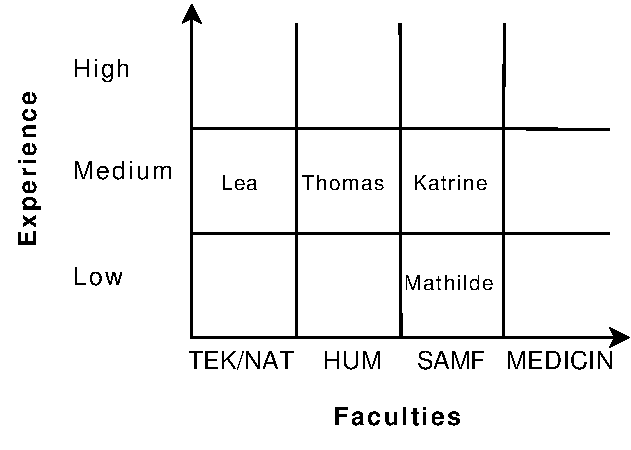
\includegraphics[width=\textwidth]{../report/images/MembersofpROJECTgROUJP.pdf}
		\label{fig:MembersofpROJECTgROUJP}
	\end{figure}
\end{frame}

\begin{frame}{\reqs}{\slutbrugere}
	\begin{itemize}
		\item Managere af projekt grupper
	\end{itemize}
	\begin{figure}
		\centering
			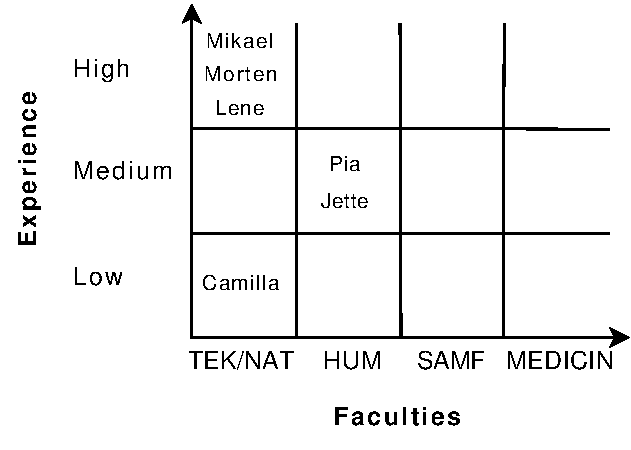
\includegraphics[width=\textwidth]{../report/images/administratorsOfPG.pdf}
		\label{fig:administratorsOfPG}
	\end{figure}
\end{frame}



\newcommand{\chosenreqs}[1]{\begin{columns}[t]
		\column{0.45\textwidth}
			\begin{itemize}
				\item \textcolor{#1}{Administrering af Projektgrupper}
				\item \textcolor{#1}{Det Virtuelle Grupperum}
				\item \textcolor{#1}{Rollebegreb}
			\end{itemize}
			
			
		\column{0.45\textwidth}
			\begin{itemize}
				\item \textcolor{#1}{Find Projektgruppe}
				\item \textcolor{#1}{Naviger til Virtuelt Grupperum}
				\item \textcolor{#1}{Pr�senter Gruppemedlemmer}
			\end{itemize}
	\end{columns}}
	
\begin{frame}{\reqs}{\funcreqs}
	\begin{itemize}
		\item \admreq
		\item \virtgrproomreq
		\item \rolereq
		\item \findgrpreq
		\item \navreq
		\item \grpmemreq
	\end{itemize}
	%Chosen
	%\only<1>{
		%\chosenreqs{black}
		%}
	%\only<2>{
		%\chosenreqs{darkgreen}
	%}
	%%Not chosen
	%\begin{columns}[t]
		%\column{0.45\textwidth}
			%\begin{itemize}
				%\item Arkivering af projektgrupper
				%\item Rekursive Projektgrupper
				%\item Administrer Roller
			%\end{itemize}
			%
		%\column{0.45\textwidth}
			%\begin{itemize}
				%\item Synkronisering af Projektgrupper
				%\item Skabeloner for Virtuelle M�desteder
			%\end{itemize}
		%
	%\end{columns}
	
\end{frame}

\begin{frame}{\reqs}{\nonfuncreqs}
	\begin{itemize}
		\item Udvidbarhed
		\item Robusthed
		\item Brugbarhed
	\end{itemize}
\end{frame}







	
	\section*{Udviklingsmetode}

\begin{frame}{Udviklingsmetode}{Udviklingsparadigme}

\begin{itemize}
	\item 
\end{itemize}

\end{frame}
%%%%%%%%%%%%%%%%%%%%%%%%%%%%%%%

\begin{frame}{Udviklingsmetode}{Valg af Agil Udviklingsmetode}



\end{frame}
%%%%%%%%%%%%%%%%%%%%%%%%%%%%%%%

\begin{frame}{Udviklingsmetode}{Tilpasning af Udviklingsmetode}
	
\end{frame}
%%%%%%%%%%%%%%%%%%%%%%%%%%%%%%%

\begin{frame}{Udviklingsmetode}{Evaluering af Udviklingsproces}
	
\end{frame}

  \newcommand{\modelreality}{Virtuelt Grupperum}
\newcommand{\topicone}{Aalborg PBL}
\newcommand{\topictwo}{Repr\ae{}sentation}
\newcommand{\topicthree}{Eksempel}
\newcommand{\topicfour}{Design}

\newcommand{\implementaras}{\modelreality}
\newcommand{\topictwoe}{Valg af Plugin Typer}
\newcommand{\topicthreee}{Context}

\section*{\modelreality}

\begin{frame}{\modelreality}
\begin{itemize}
	\item Analyse
	
	\begin{itemize}
		\item \topicone
		\item \topictwo
  \end{itemize}
	
	\item \topicfour
	\begin{itemize}

		\item \topictwoe
		\item \topicthreee
	\end{itemize}
	\item Implementation
  \begin{itemize}
		\item Standard Projekt V�rkt�jer
	\end{itemize}

\end{itemize}
\end{frame}

\begin{frame}{\modelreality}{Analyse} 

\begin{center}
\huge Analyse
\end{center}

\end{frame}

\begin{frame}{\modelreality}{\topicone}
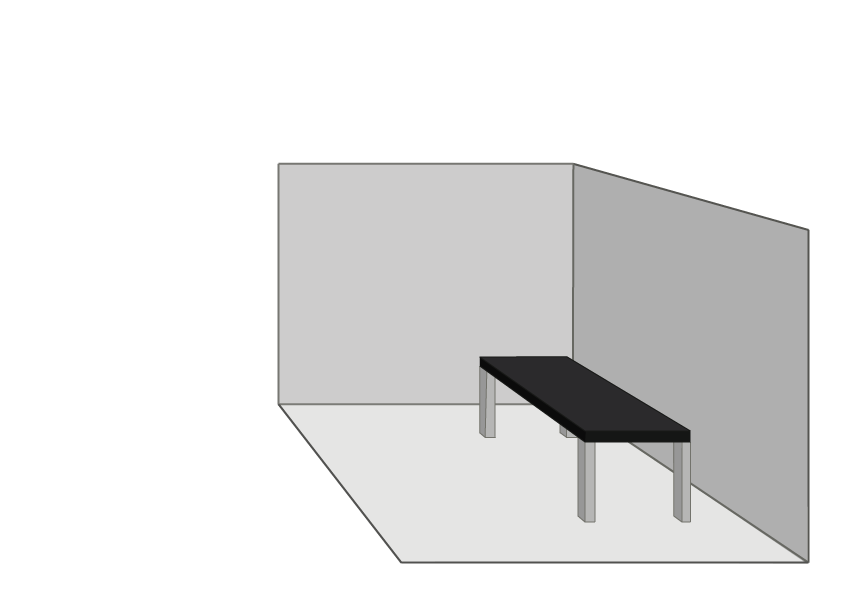
\includegraphics[width=\columnwidth]{input/rasmus/ras5.png}
\end{frame}
\begin{frame}{\modelreality}{\topicone} 
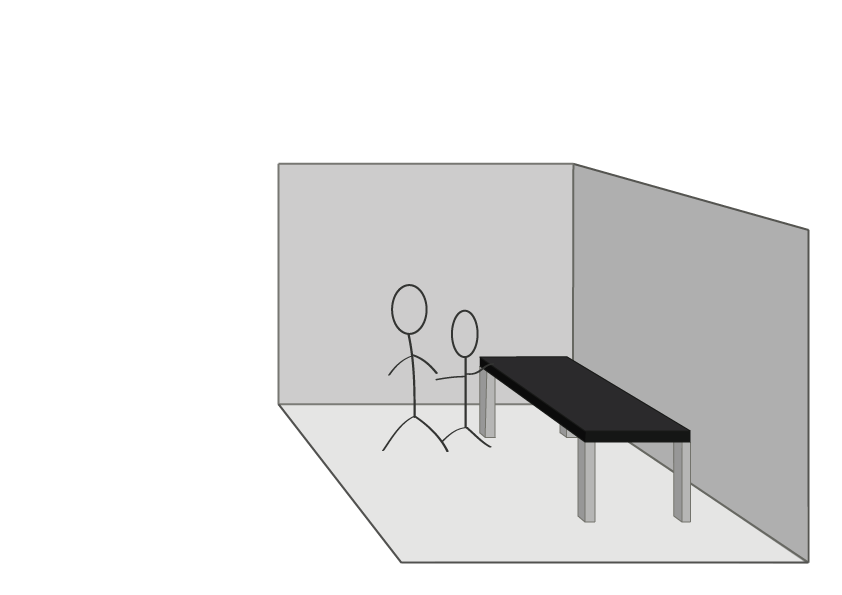
\includegraphics[width=\columnwidth]{input/rasmus/ras4.png}
\end{frame}
\begin{frame}{\modelreality}{\topicone} 
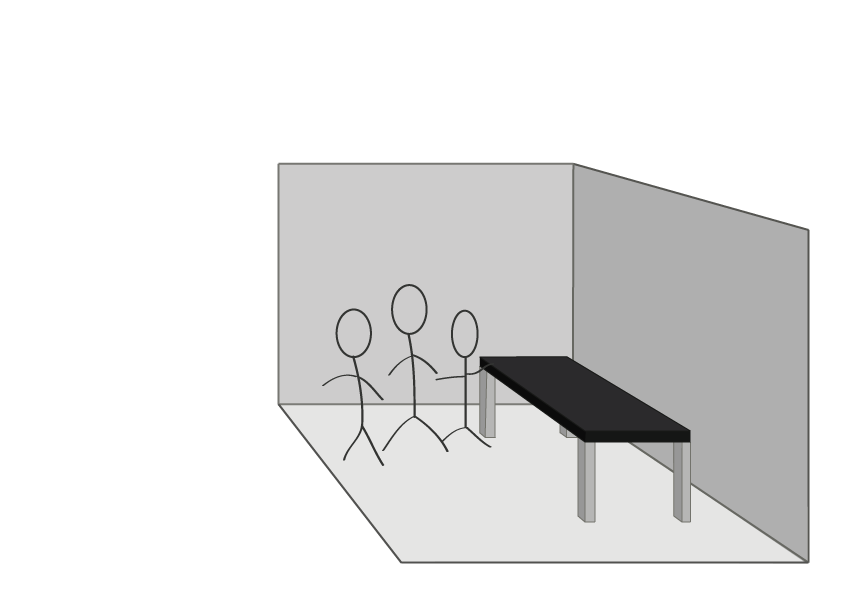
\includegraphics[width=\columnwidth]{input/rasmus/ras3.png}
\end{frame}
\begin{frame}{\modelreality}{\topicone} 
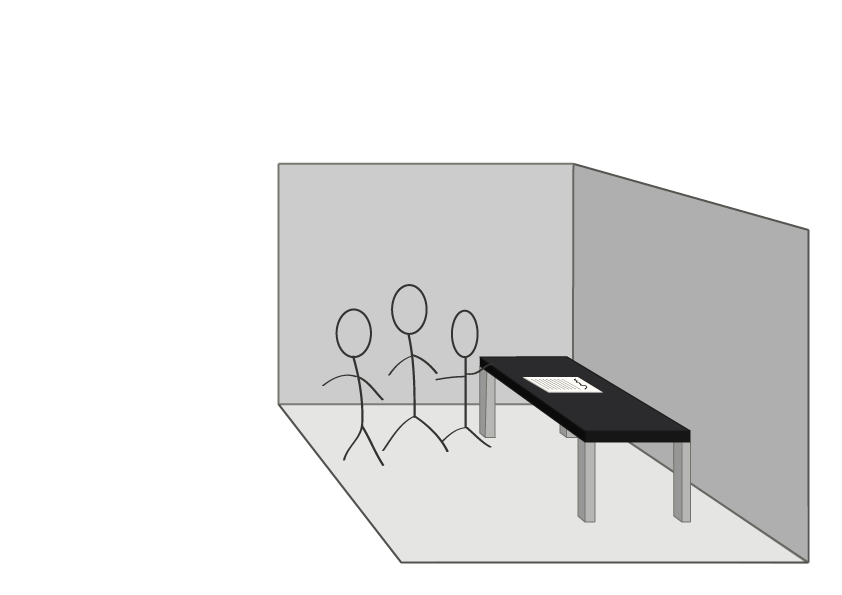
\includegraphics[width=\columnwidth]{input/rasmus/ras2.png}
\end{frame}
\begin{frame}{\modelreality}{\topicone} 
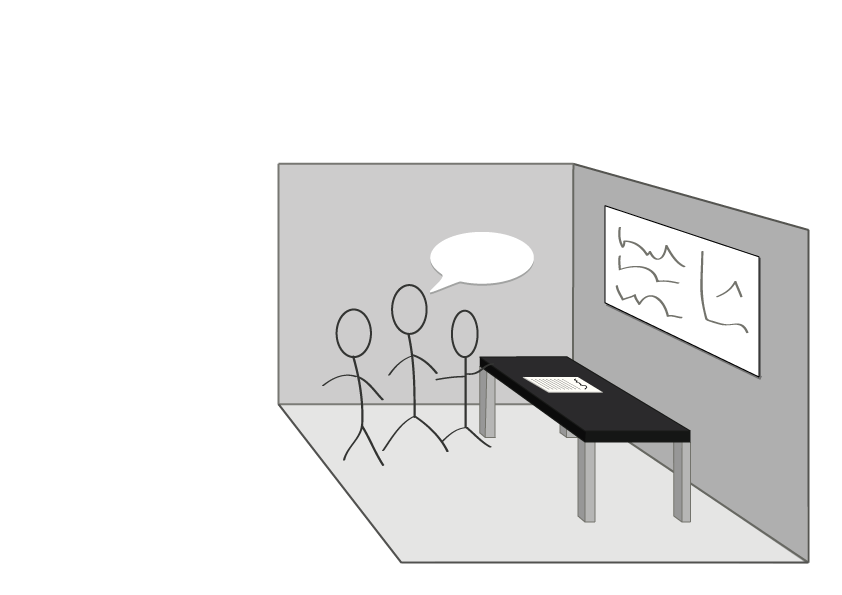
\includegraphics[width=\columnwidth]{input/rasmus/ras1.png}
\end{frame}


\def\freqlist{1,2,3}

\foreach \freq in \freqlist 
{
\begin{frame}{\modelreality}{\topictwo} 
\begin{figure}
\includegraphics[width=\columnwidth]{input/rasmus/two\freq.pdf}
\end{figure}
\end{frame}

} 

\def\freqlist{4,5,6}

\foreach \freq in \freqlist 
{
\begin{frame}{\modelreality}{\topicthree} 
\begin{figure}
\includegraphics[width=\columnwidth]{input/rasmus/two\freq.pdf}
\end{figure}
\end{frame}

} 

\def\freqlist{7,8,9}

\foreach \freq in \freqlist 
{
\begin{frame}{\modelreality}{\topictwo} 
\begin{figure}
\includegraphics[width=\columnwidth]{input/rasmus/two\freq.pdf}
\end{figure}
\end{frame}

} 

\begin{frame}{\modelreality}{\topicfour} 

\begin{center}
\huge Design
\end{center}

\end{frame}


\begin{frame}{\modelreality}{\topicfour} 
\begin{figure}
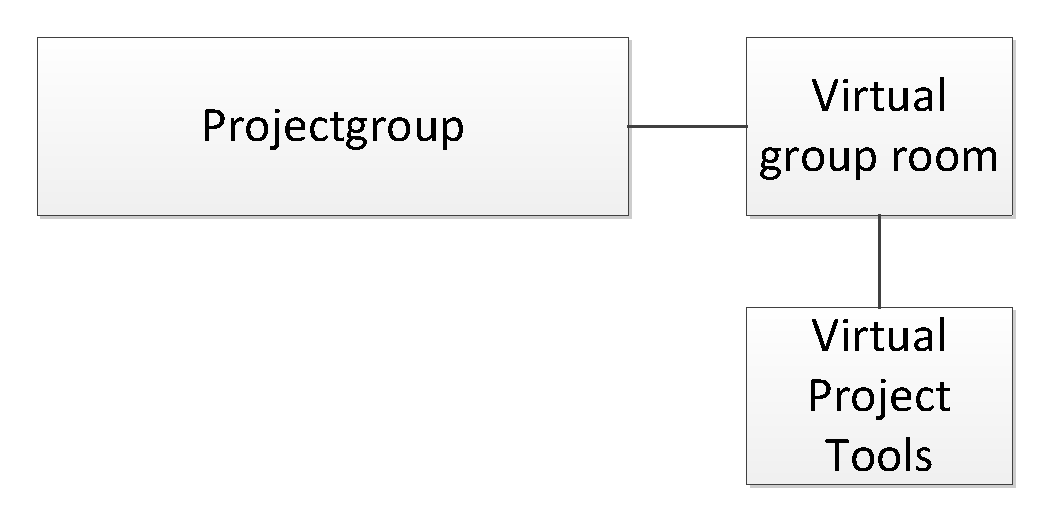
\includegraphics[width=\columnwidth]{input/rasmus/two10.pdf}
\end{figure}
\end{frame}

\begin{frame}{\modelreality}{\topicfour} 
\begin{figure}
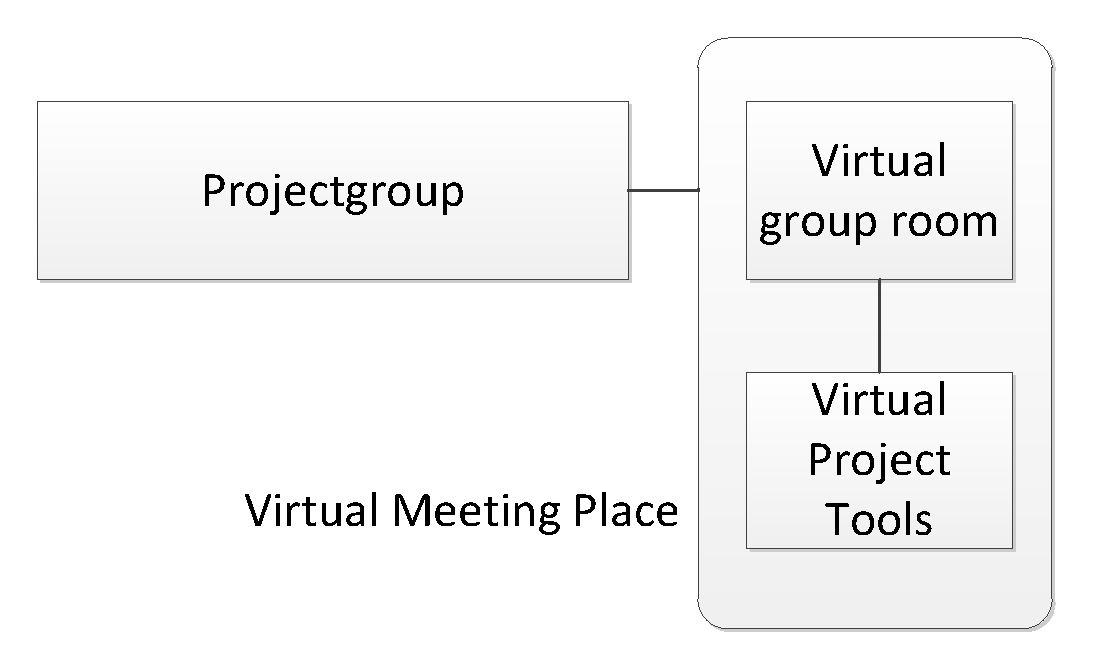
\includegraphics[width=\columnwidth]{input/rasmus/two11.pdf}
\end{figure}
\end{frame}



\def\freqlist{1,1a,2,3,4,5,6,7,7a,8}

\foreach \freq in \freqlist 
{
\begin{frame}{\implementaras} {\topictwoe}
\begin{figure}
\includegraphics[width=\columnwidth]{input/rasmus/three\freq.pdf}
\end{figure}
\end{frame}
}

\def\freqlist{9}

\foreach \freq in \freqlist 
{
\begin{frame}{\implementaras}{\topicthreee} 
\begin{figure}
\includegraphics[width=\columnwidth]{input/rasmus/three\freq.pdf}
\end{figure}
\end{frame}
} 


\begin{frame}{\implementaras}{\topicthreee}
\begin{figure}
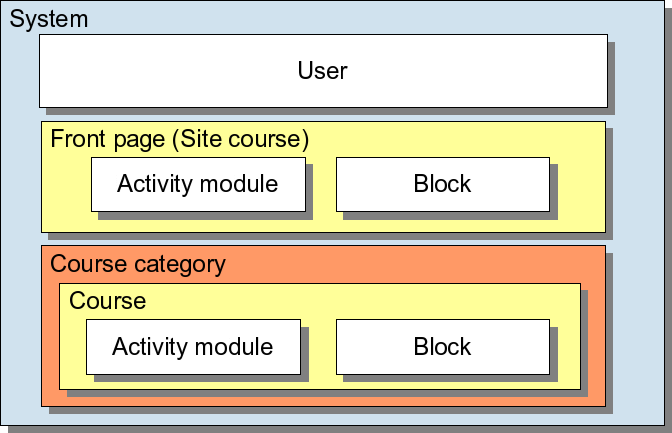
\includegraphics[width=\columnwidth]{input/rasmus/Moodle-contexts.png}
\end{figure}
\end{frame}

\begin{frame}{\implementaras}{\topicthreee}
\begin{figure}
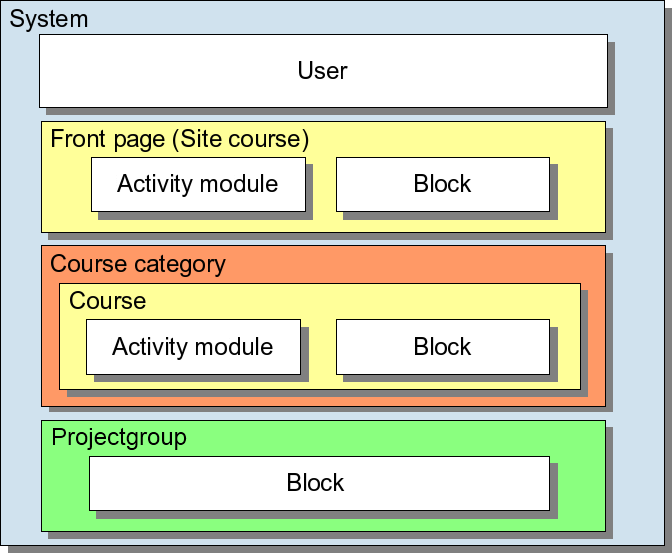
\includegraphics[width=\columnwidth]{input/rasmus/Moodle-contexts-mymoodle.png}
\end{figure}
\end{frame}


\begin{frame}{\modelreality}{Implementation} 

\begin{center}
\huge Implementation
\end{center}

\end{frame}
\end{document}
